In this section, we will explain our findings for buildings across different campuses. As per our previous shown data analysis, buildings with the supply-demand problems as shown in the below figure are analyzed. Those buildings are also chosen because of their higher floor levels. Hence, we have a better prediction when different factors are incorporated. We have completed the analysis for the following buildings:

\begin{itemize}
    \item Doug McDonell Building, Parkville (168)  - Appendix Table \ref{appendix:doug_mr_floor}
    \item Alan Gilbert Building, Parkville (104) - Appendix Table \ref{appendix:alan_mr_floor}
    \item Law Building, Parkville (106) - Appendix Table \ref{appendix:law_mr_floor}
    \item Stop 1 Building, Parkville (199) - Appendix Table \ref{appendix:stop1_mr_floor}
    \item 100 Leicester St, Parkville (278) - Appendix Table \ref{appendix:edu_mr_floor}
    \item Glyn Davis Building, Parkville (133) - Appendix Table \ref{appendix:glyn_mr_floor}
    \item Elisabeth Murdoch Building, Southbank (860) - Appendix Table \ref{appendix:eliz_mr_floor}
    \item Werribee Veterinary Hospital, Werribee (411) - Appendix Table \ref{appendix:werribee_mr_floor}
\end{itemize}

\begin{figure}[H]
\centering
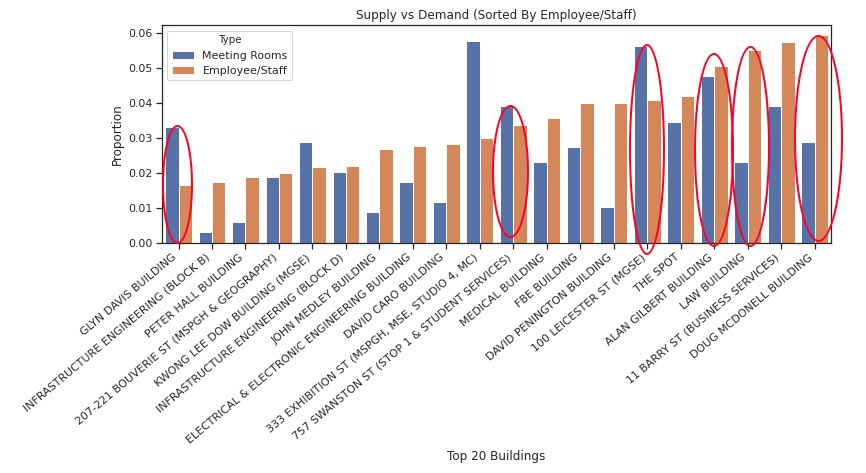
\includegraphics[width=10cm,keepaspectratio=true]{content/results/floors/plots/Building.png}
\caption{Supply vs Demand Problem in Parkville Campus}
\label{fig:Building}
\end{figure}

% \paragraph{Doug McDonell Building (Parkville Campus)}

% In this section, we will explain our findings of Doug McDonell Building from the perspective of supply and demand analysis.

% \begin{itemize}
%     \item \textbf{Best nearby floors with no preference:} As shown in the Appendix Table \ref{appendix:doug_mr_floor}, a staff member needs to walk at least \texttt{3 levels} (Budget) in Doug McDonell Building to get rewarding floors with an adequate supply of meeting rooms. We also suggest a relaxing budget ($\delta$) of \texttt{4 levels} so that employee doesn't miss out on a high supply providing floors. Using these constraints, we suggest \texttt{level 8} as the most rewarding floor with the cost of \texttt{7 floors} followed by \texttt{level 4} with \texttt{3 floors} and \texttt{level 7} with \texttt{6 floors} as shown in the Figure \ref{fig:doug-floor-no-factors}.
    
    


% \begin{figure}[H]

% \centering
%   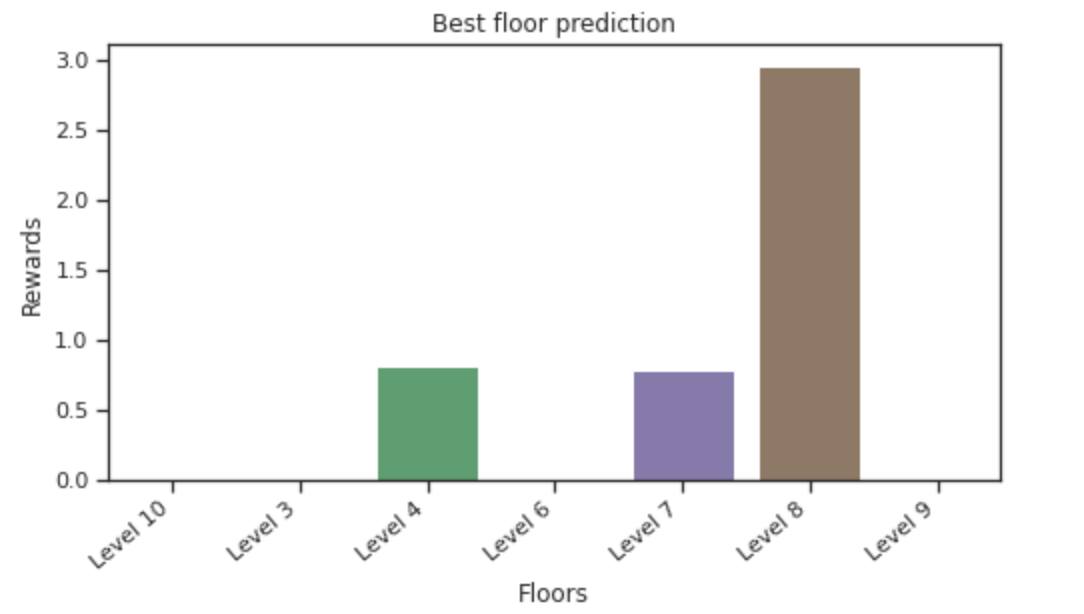
\includegraphics[width=8cm]{content/results/floors/plots/doug-floor-no-factors.png}
  
% \caption{Best rewarding floors from Doug McDonell}
% \label{fig:doug-floor-no-factors}
% \end{figure}

% \item \textbf{Best nearby floors under COVID-19 Strict Lockdown:} As shown in the Appendix Table \ref{appendix:doug_mr_floor} with COVID-19 high factor, a staff member should be willing to walk at least \texttt{5 levels} (Budget) in Doug McDonell Building to get very high rewarding floors under COVID-19 lockdown with the relaxing budget($\delta$) of at least \texttt{2 levels}. Using these constraints, we suggest \texttt{level 8} as the most rewarding floor with the cost of \texttt{7 floors} followed by \texttt{level 7} with \texttt{6 floors} and \texttt{level 5} with \texttt{4 floors} as shown in the Figure \ref{fig:doug-floor-covid}.

% \begin{figure}[H]
% \centering
%   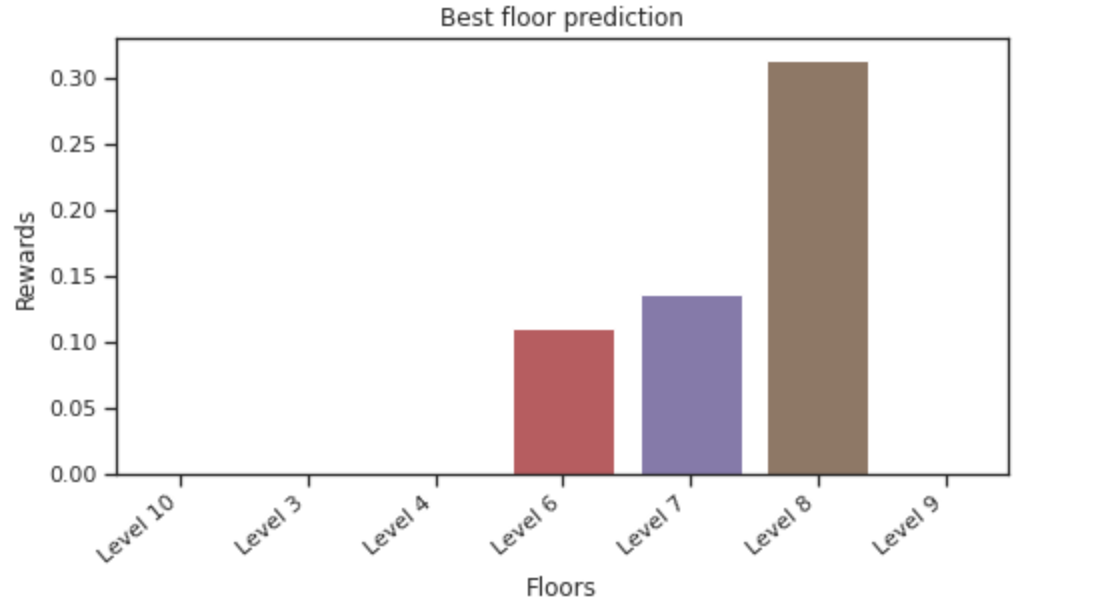
\includegraphics[width=8cm]{content/results/floors/plots/doug-floor-covid.png}
  
% \caption{Best rewarding floors from Doug McDonell with COVID lockdown}
% \label{fig:doug-floor-covid}
% \end{figure}

% \item \textbf{Best nearby floors with High Capacity:} As shown in the Appendix Table \ref{appendix:doug_mr_floor} with high capacity factor, a staff member can easily find a high supply of meeting rooms providing floors in Doug McDonell building within the budget of \texttt{3 levels } and relaxing budget($\delta$) of at least \texttt{4 levels}. Using these constraints, we again suggest \texttt{level 8} as the most rewarding floor with the cost of \texttt{7 floors} followed by \texttt{level 4} with \texttt{3 floors} and \texttt{level 7} with \texttt{6 floors} as shown in the Figure \ref{fig:doug-floor-capacity}.

% \begin{figure}[H]
% \centering
%   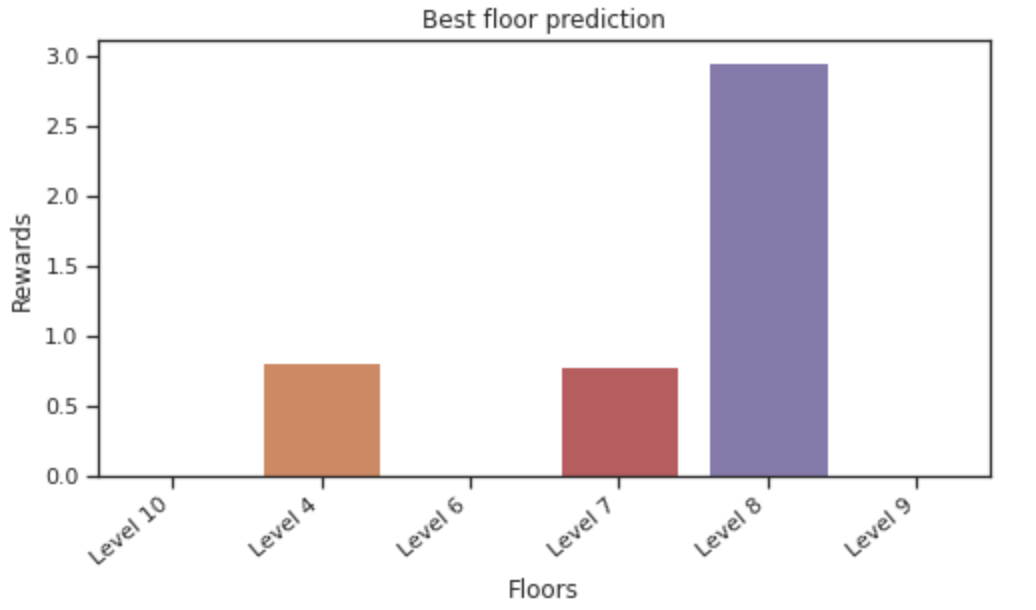
\includegraphics[width=8cm]{content/results/floors/plots/doug-floor-capacity.png}
% \caption{Best rewarding floors from Doug McDonell with high capacity}
% \label{fig:doug-floor-capacity}
% \end{figure}

% \item \textbf{Best nearby floors with other factors:} In the appendix Table \ref{appendix:doug_mr_floor}, we have also shown other factors such as finding meeting rooms with equipment, excellent conditions, and easy availability with their budgets and relaxing budgets. Using those constraints, we suggest that \texttt{level 8} is the most rewarding floor for meeting rooms with equipment and finding meeting rooms in excellent condition. \texttt{level 4} is the most rewarding floor for finding meeting rooms which are easily available.

% The results are summarized below using floors bar chart for different factors.

% \begin{figure}[H]
% \centering
% \begin{subfigure}[b]{0.30\textwidth}
%   \centering
%   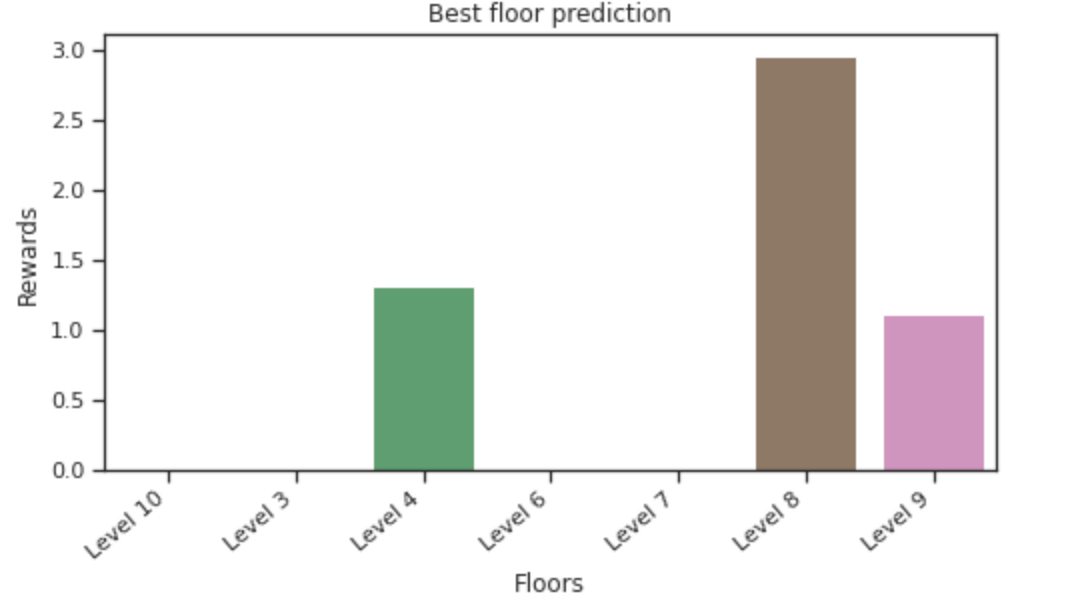
\includegraphics[width=5.5cm,keepaspectratio=true]{content/results/floors/plots/doug-floor-equipment.png}
% \end{subfigure}
% \begin{subfigure}[b]{0.30\textwidth}
%   \centering
%   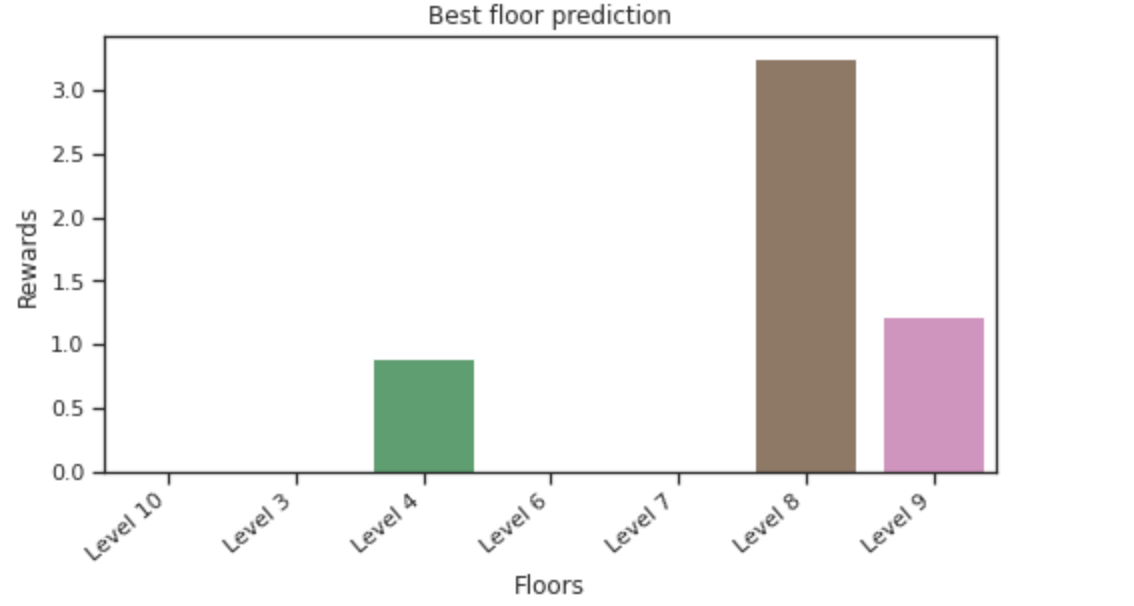
\includegraphics[width=5.5cm,keepaspectratio=true]{content/results/floors/plots/doug-floor-excellent.png}
% \end{subfigure}
% \begin{subfigure}[b]{0.30\textwidth}
%   \centering
%   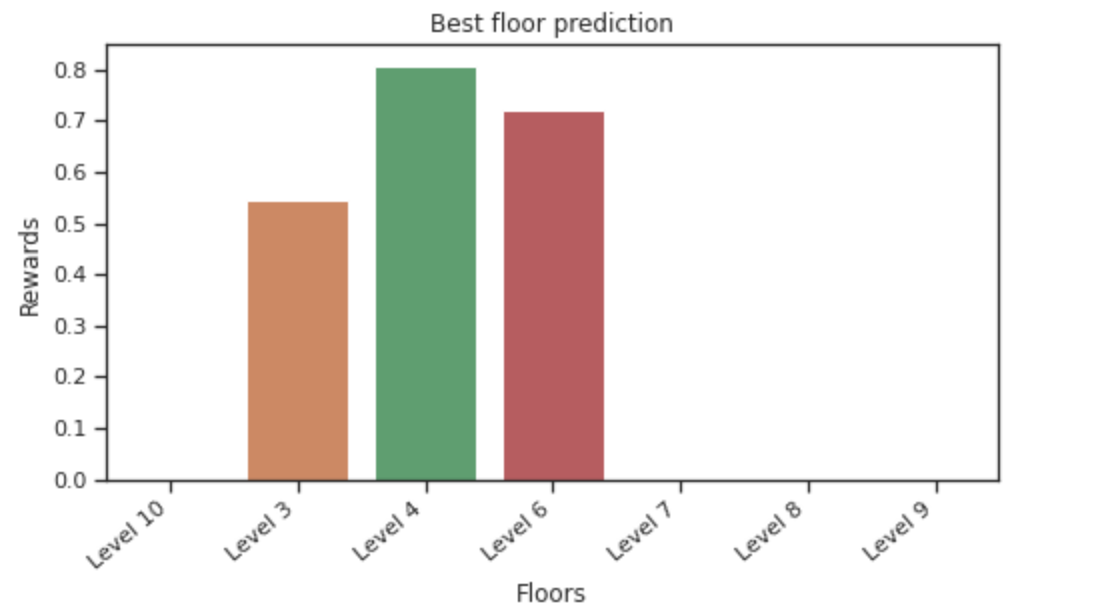
\includegraphics[width=5.5cm,keepaspectratio=true]{content/results/floors/plots/doug-floor-available.png}
% \end{subfigure}
% \caption{Best rewarding floors of nearby floors from Doug McDonell based on different factors}
% \label{fig:doug-floor-other-factors}
% \end{figure}
% \end{itemize}


\paragraph{Alan Gilbert Building (Parkville Campus)}
In this section, we will explain our findings of Alan Gilbert Building from the perspective of supply and demand analysis.

\begin{itemize}
    \item \textbf{Best nearby floors with no preference:} As shown in the Appendix Table \ref{appendix:alan_mr_floor}, a staff member needs to walk at least \texttt{1 level} (Budget) in Alan Gilbert Building to get rewarding floors with an adequate supply of meeting rooms. We also suggest a relaxing budget ($\delta$) of \texttt{3 levels} so that employee doesn't miss out on a high supply providing floors. Using these constraints, we suggest \texttt{level 5} as the most rewarding floor with the cost of \texttt{4 floors} followed by \texttt{level 4} with \texttt{3 floors} and \texttt{level 2} with \texttt{1 floor} as shown in the Figure \ref{fig:alan-floor-no-factors}.

\begin{figure}[H]
\centering
  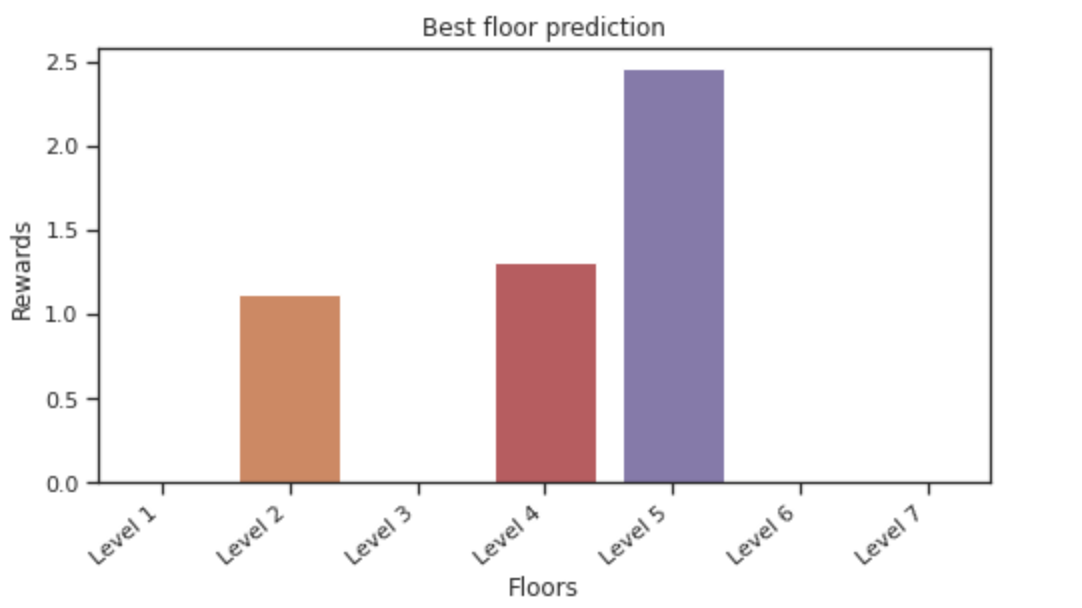
\includegraphics[width=8cm]{content/results/floors/plots/alan-floor-no-factors.png}
\caption{Best rewarding floors from Alan Gilbert}
\label{fig:alan-floor-no-factors}
\end{figure}
    
\item \textbf{Best nearby floors under COVID-19 Strict Lockdown:} As shown in the Appendix Table \ref{appendix:alan_mr_floor} with COVID-19 high factor, a staff member needs to walk at least \texttt{1 level} (Budget) in Alan Gilbert Building to get rewarding floors under  COVID-19 lockdown with the relaxing budget ($\delta$) of \texttt{3 levels} so that employee doesn't miss out a high supply providing floors. Using these constraints, we suggest \texttt{level 5} as the most rewarding floor with the cost of \texttt{4 floors} followed by \texttt{level 4} with \texttt{3 floors} and \texttt{level 2} with \texttt{1 floor} as shown in the Figure \ref{fig:alan-floor-covid}.

\begin{figure}[H]
\centering
  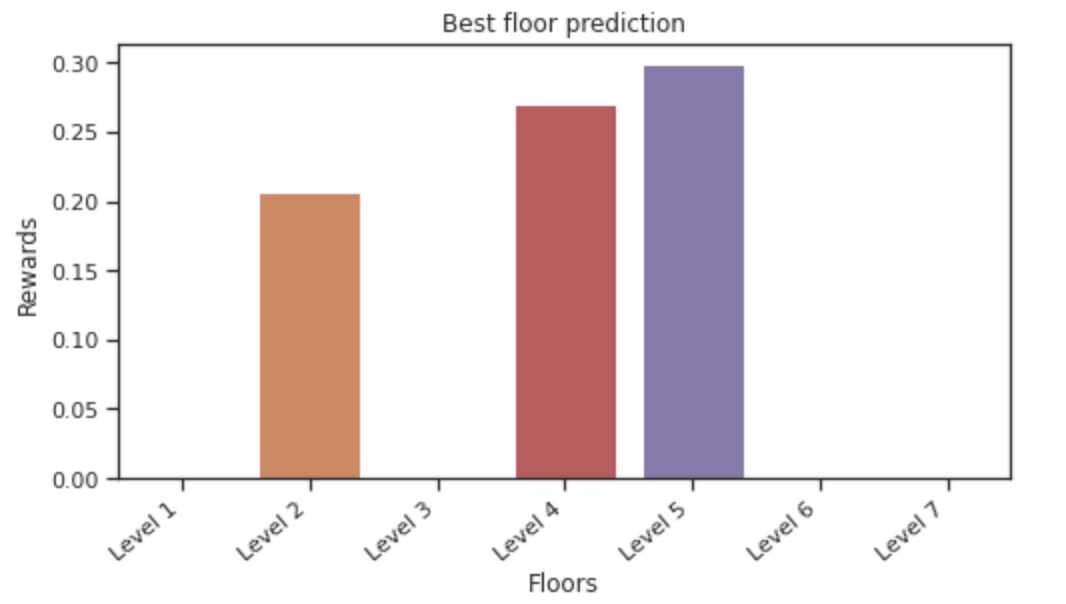
\includegraphics[width=8cm]{content/results/floors/plots/alan-floor-covid.png}
\caption{Best rewarding floors from Alan Gilbert with COVID lockdown}
\label{fig:alan-floor-covid}
\end{figure}
    
% \item \textbf{Best nearby floors with excellent room condition:} As shown in the Appendix Table \ref{appendix:alan_mr_floor} with excellent room condition factor, a staff member needs to walk at least \texttt{3 level} (Budget) in Alan Gilbert Building to get rewarding floors to have an excellent meeting room with the relaxing budget ($\delta$) of \texttt{3 levels} so that employee doesn't miss out a high supply providing floors. Using these constraints, we suggest \texttt{level 5} as the most rewarding floor with the cost of \texttt{4 floors} followed by \texttt{level 4} with \texttt{3 floors} and \texttt{level 7} with \texttt{6 floors} as shown in the Figure \ref{fig:alan-floor-excellent}.

%\begin{figure}[H]
%\centering
%  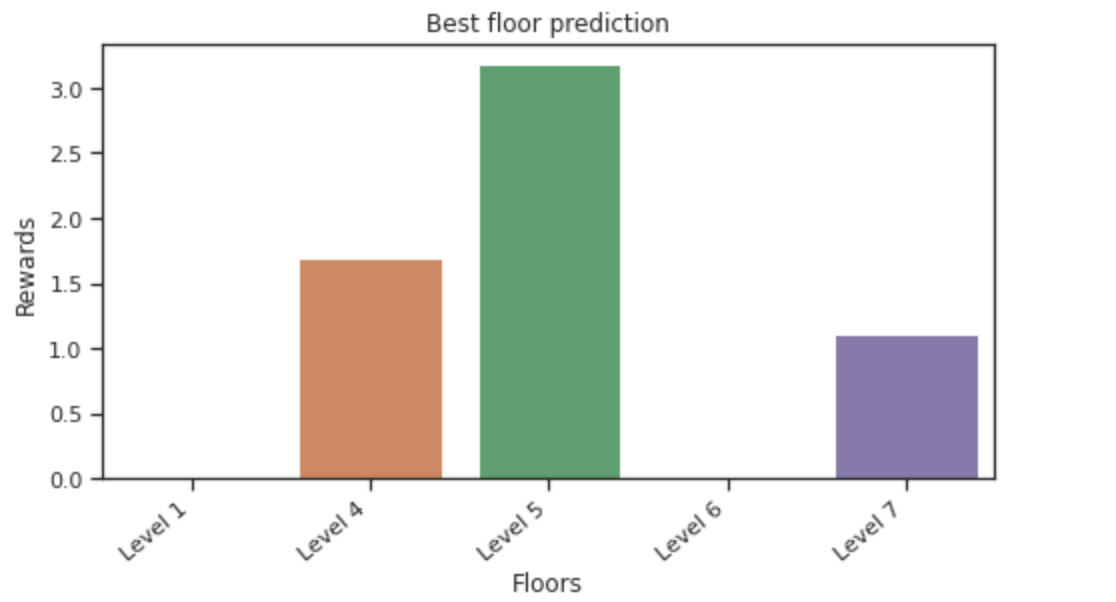
\includegraphics[width=8cm]{content/results/floors/plots/alan-floor-excellent.png}
%\caption{Best rewarding floors from Alan Gilbert with excellent room condition}
%\label{fig:alan-floor-excellent}
%\end{figure}


\item \textbf{Best nearby floors with other factors:} In the appendix Table \ref{appendix:alan_mr_floor}, we have also shown other factors such as finding meeting rooms with high capacity, equipment, and easy availability with their budgets and relaxing budgets. Using those constraints, we suggest that \texttt{level 5} is the most rewarding floor for all those factors.



\begin{figure}[H]
\centering
  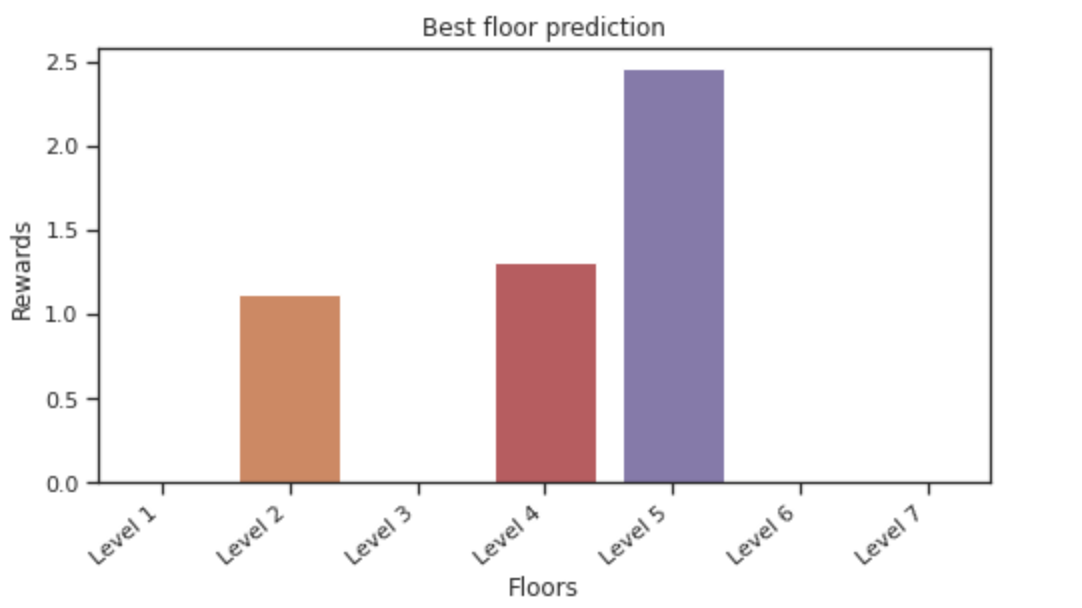
\includegraphics[width=8cm]{content/results/floors/plots/alan-floor-no-factors.png}
  
\caption{Best rewarding floors from Alan Gilbert with other factors}
\label{fig:alan-floor-other-factors}
\end{figure}

\end{itemize}


\paragraph{Law Building (Parkville Campus)}
In this section, we will explain our findings of Law Building from the perspective of supply and demand analysis.

\begin{itemize}
    \item \textbf{Best nearby floors with no preference:} As shown in the Appendix Table \ref{appendix:law_mr_floor}, a staff member needs to walk at least \texttt{1 level} (Budget) in Law Building to get rewarding floors with an adequate supply of meeting rooms. We also suggest a relaxing budget ($\delta$) of \texttt{4 levels} so that employee doesn't miss out on a high supply providing floors. Using these constraints, we suggest \texttt{level 2} as the most rewarding floor with the cost of \texttt{1 floor} followed by \texttt{level 3} with \texttt{2 floors} and \texttt{level 6} with \texttt{5 floors} as shown in the Figure \ref{fig:law-floor-no-factors}.

\begin{figure}[H]
\centering
  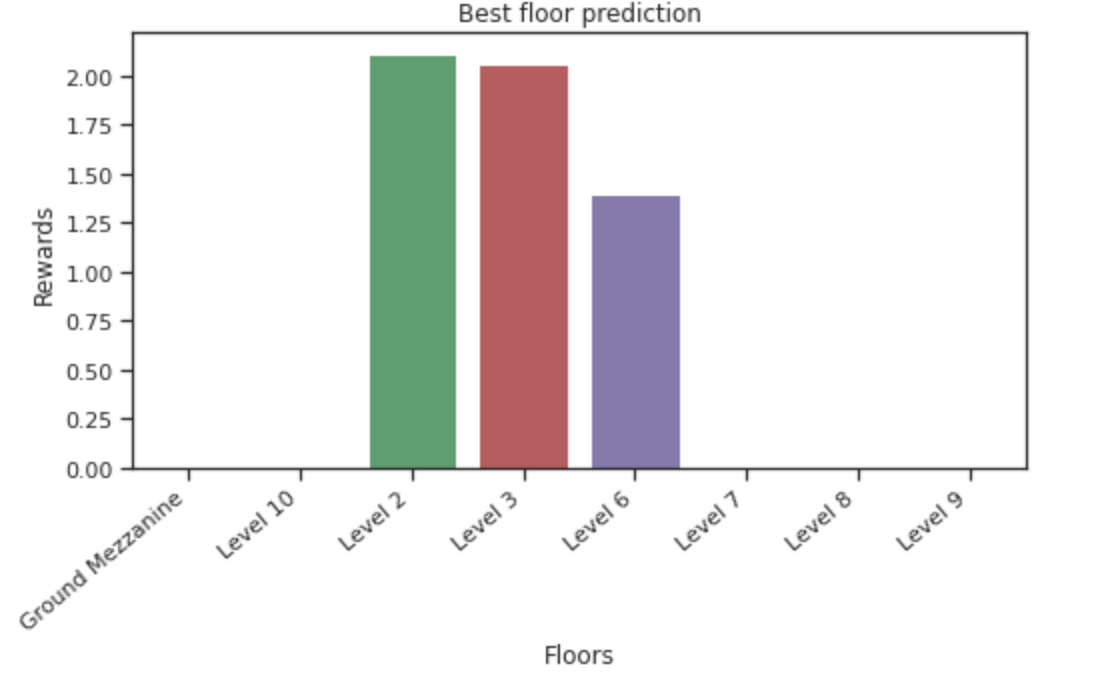
\includegraphics[width=8cm]{content/results/floors/plots/law-floor-no-factors.png}
\caption{Best rewarding floors from Law Building}
\label{fig:law-floor-no-factors}
\end{figure}

%\item \textbf{Best nearby floors under COVID-19 Strict Lockdown:} As shown in the Appendix Table \ref{appendix:law_mr_floor} with COVID-19 high factor, a staff member needs to walk at least \texttt{1 level} (Budget) in Law Building to get rewarding floors under  COVID-19 lockdown with the relaxing budget ($\delta$) of \texttt{2 levels} so that employee doesn't miss out a high supply providing floors. Using these constraints, we suggest \texttt{Ground Mezzanine} as the most rewarding floor with the cost of \texttt{0.5 floor} followed by \texttt{level 2} with \texttt{1 floor} and \texttt{level 3} with \texttt{2 floors} as shown in the Figure \ref{fig:law-floor-covid}.

%\begin{figure}[H]
%\centering
%  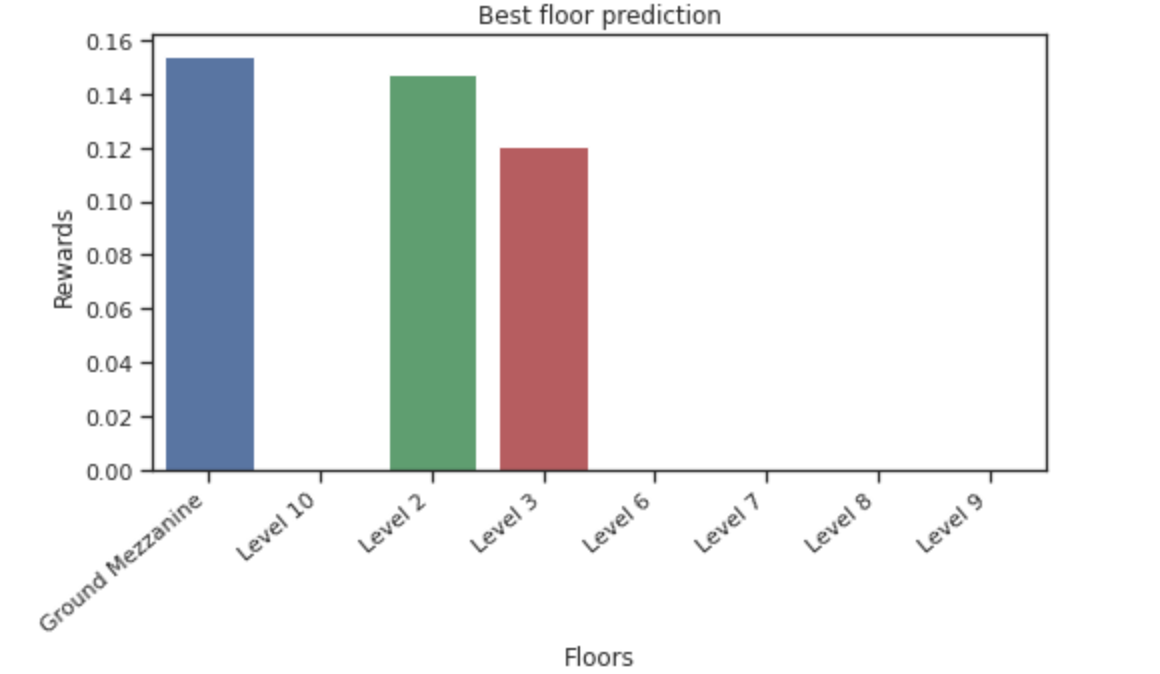
\includegraphics[width=8cm]{content/results/floors/plots/law-floor-covid.png}
%\caption{Best rewarding floors from Law with COVID lockdown}
%\label{fig:law-floor-covid}
%\end{figure}

\item \textbf{Best nearby floors with equipment:} As shown in the Appendix Table \ref{appendix:law_mr_floor} with equipment factor, a staff member needs to walk at least \texttt{1 level} (Budget) in Law  Building to get rewarding floors to have an excellent meeting room with a relaxing budget ($\delta$) of \texttt{4 levels} so that employee doesn't miss out a high supply providing floors. Using these constraints, we suggest \texttt{level 6} as the most rewarding floor with the cost of \texttt{5 floors} followed by \texttt{level 2} with \texttt{1 floor} and \texttt{level 3} with \texttt{2 floors} as shown in the Figure \ref{fig:law-floor-equipment}.

\begin{figure}[H]
\centering
  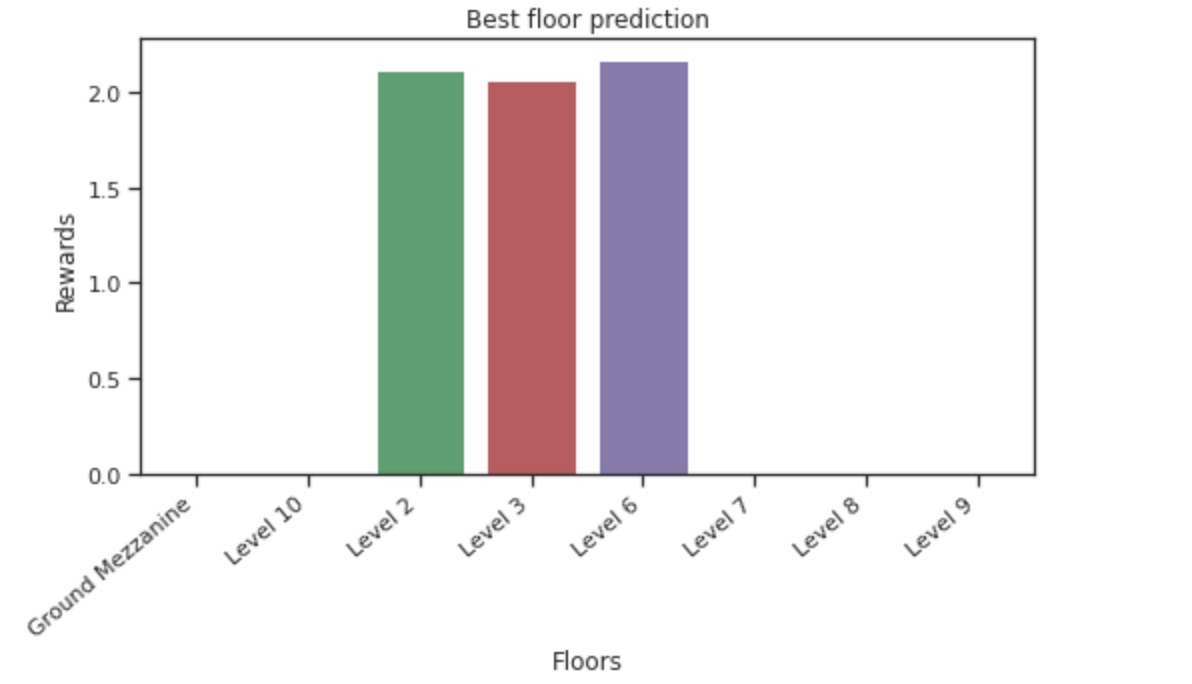
\includegraphics[width=8cm]{content/results/floors/plots/law-floor-equipment.png}
\caption{Best rewarding floors from Law with equipment}
\label{fig:law-floor-equipment}
\end{figure}

\item \textbf{Best nearby floors with other factors:} In the appendix Table \ref{appendix:law_mr_floor}, we have also shown other factors such as finding meeting rooms with high capacity, excellent room condition, and easy availability with their budgets and relaxing budgets. Using those constraints, we suggest that \texttt{level 2} is the most rewarding floor for all those factors.

\begin{figure}[H]
\centering
  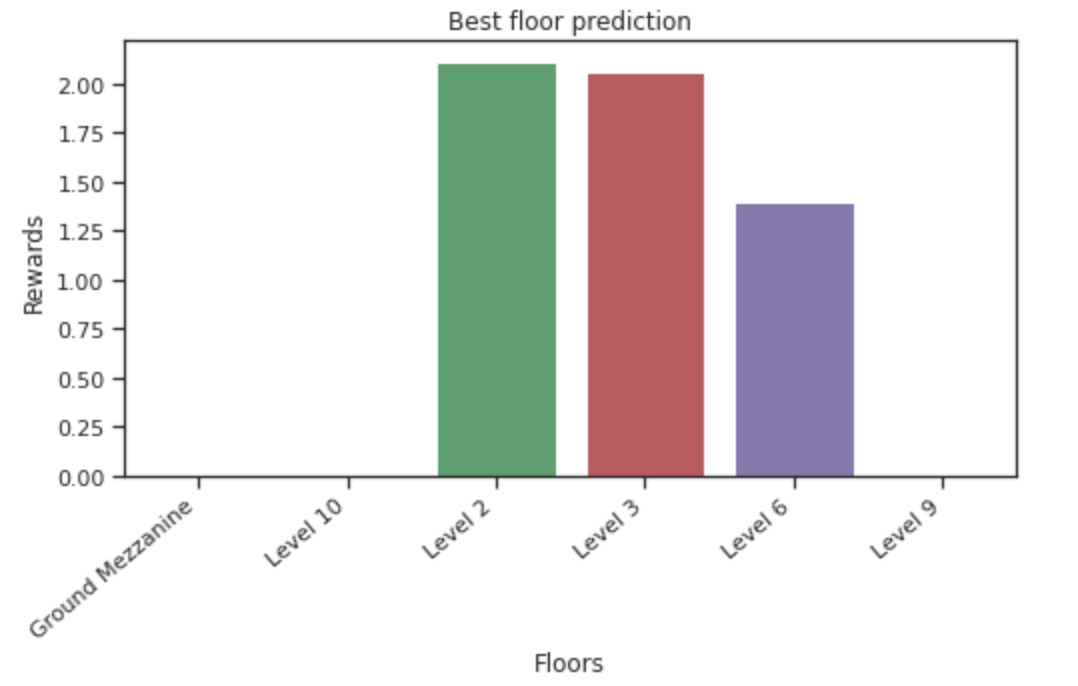
\includegraphics[width=8cm]{content/results/floors/plots/law-floor-capacity.png}
\caption{Best rewarding floors from Law with other factors}
\label{fig:law-floor-capacity}
\end{figure}

\end{itemize}


% \paragraph{Stop1 Building (Parkville Campus)}
% In this section, we will explain our findings of Stop 1 Building from the perspective of supply and demand analysis.

% \begin{itemize}
%     \item \textbf{Best nearby floors with no preference:} As shown in the Appendix Table \ref{appendix:stop1_mr_floor}, a staff member needs to walk at least \texttt{1 level} (Budget) in Stop1 Building to get rewarding floors with an adequate supply of meeting rooms. We also suggest a relaxing budget ($\delta$) of \texttt{4 levels} so that employee doesn't miss out on a high supply providing floors. Using these constraints, we suggest \texttt{level 6} as the most rewarding floor with the cost of \texttt{5 floors} followed by \texttt{level 5} with \texttt{4 floors} and \texttt{level 2} with \texttt{1 floor} as shown in the Figure \ref{fig:stop1-floor-no-factors}.

% \begin{figure}[H]
% \centering
%   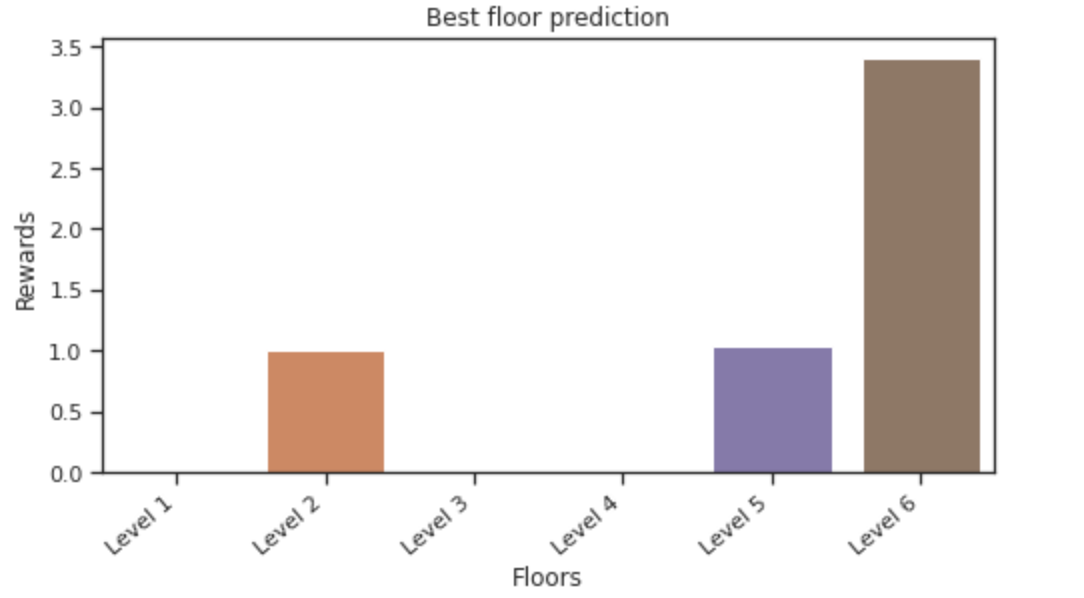
\includegraphics[width=8cm]{content/results/floors/plots/stop1-floor-no-factors.png}
% \caption{Best rewarding floors from Stop1 Building}
% \label{fig:stop1-floor-no-factors}
% \end{figure}

% \item \textbf{Best nearby floors under COVID-19 Strict Lockdown:} As shown in the Appendix Table \ref{appendix:stop1_mr_floor} with COVID-19 high factor, a staff member needs to walk at least \texttt{1 level} (Budget) in Stop1 Building to get rewarding floors under  COVID-19 lockdown with the relaxing budget ($\delta$) of \texttt{3 levels} so that employee doesn't miss out a high supply providing floors. Using these constraints, we suggest \texttt{level 4} as the most rewarding floor with the cost of \texttt{3 floors} followed by \texttt{level 5} with \texttt{4 floors} and \texttt{level 2} with \texttt{1 floor} as shown in the Figure \ref{fig:stop1-floor-covid}.

% \begin{figure}[H]
% \centering
%   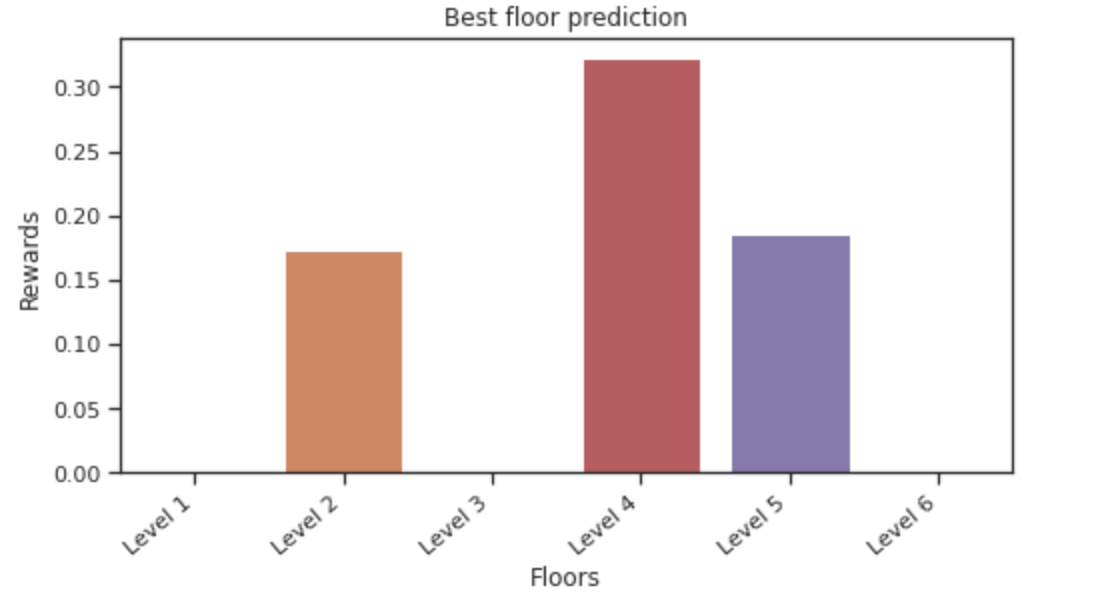
\includegraphics[width=8cm]{content/results/floors/plots/stop1-floor-covid.png}
% \caption{Best rewarding floors from Stop1 with COVID lockdown}
% \label{fig:stop1-floor-covid}
% \end{figure}

% \item \textbf{Best nearby floors with equipment:} As shown in the Appendix Table \ref{appendix:stop1_mr_floor} with equipment factor, a staff member needs to walk at least \texttt{3 levels} (Budget) in Stop1  Building to get rewarding floors to have an excellent meeting room with a relaxing budget ($\delta$) of \texttt{2 levels} so that employee doesn't miss out a high supply providing floors. Using these constraints, we suggest \texttt{level 6} as the most rewarding floor with the cost of \texttt{5 floors} followed by \texttt{level 4} with \texttt{3 floors} and \texttt{level 5} with \texttt{4 floors} as shown in the Figure \ref{fig:stop1-floor-equipment}.

% \begin{figure}[H]
% \centering
%   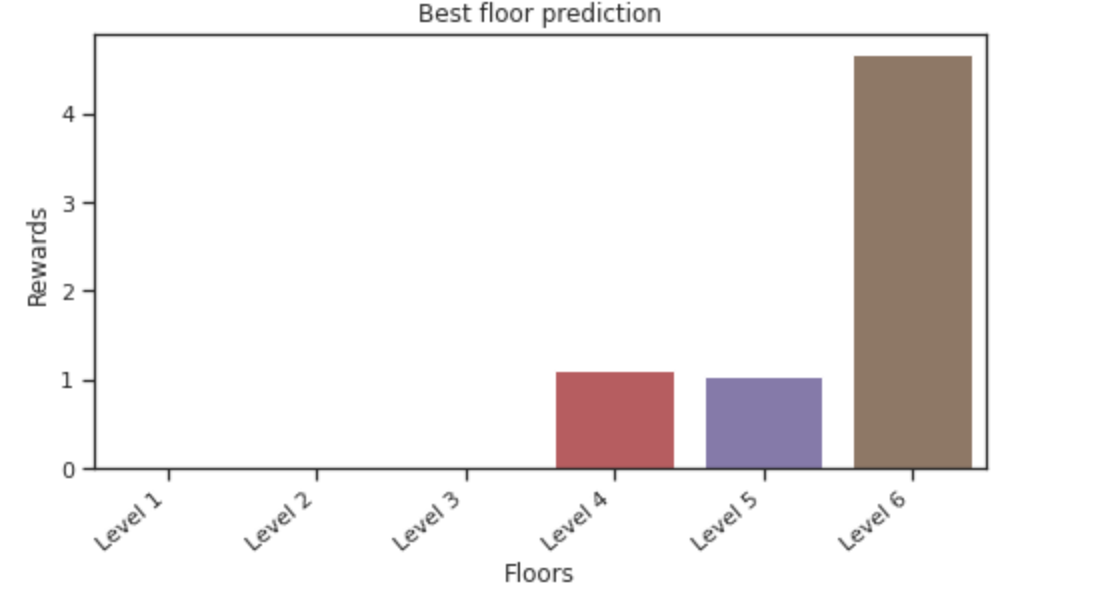
\includegraphics[width=8cm]{content/results/floors/plots/stop1-floor-equipment.png}
% \caption{Best rewarding floors from Stop1 with equipment}
% \label{fig:stop1-floor-equipment}
% \end{figure}

% \item \textbf{Best nearby floors with other factors:} In the appendix Table \ref{appendix:stop1_mr_floor}, we have also shown other factors such as finding meeting rooms with high capacity, excellent room condition, and easy availability with their budgets and relaxing budgets. Using those constraints, we suggest that \texttt{level 6} is the most rewarding floor for all those factors.

% \begin{figure}[H]
% \centering
%   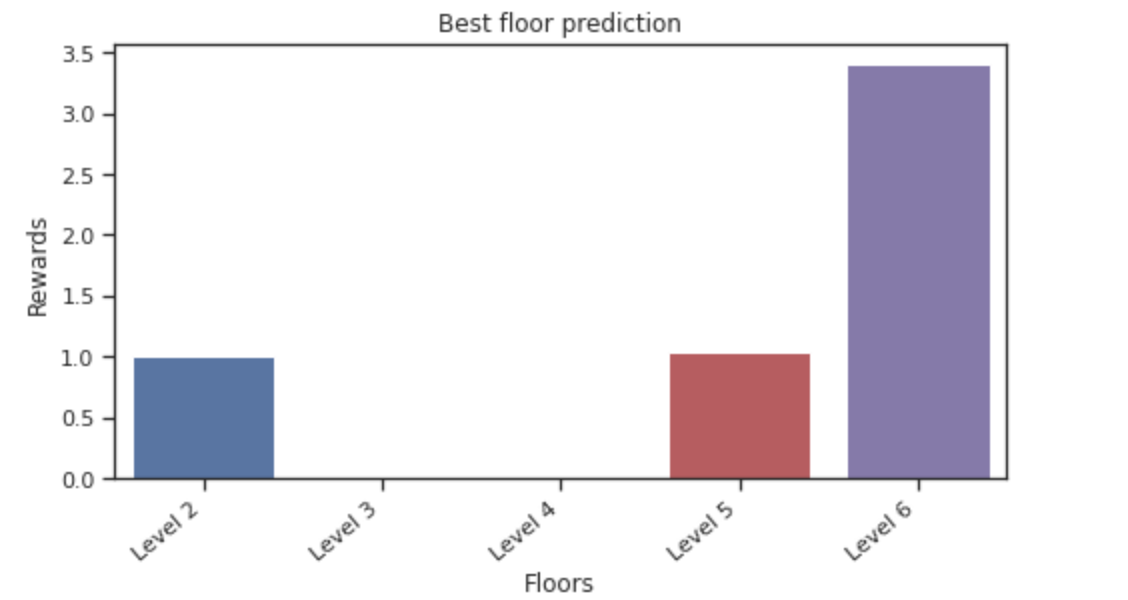
\includegraphics[width=8cm]{content/results/floors/plots/stop1-floor-capacity.png}
% \caption{Best rewarding floors from Stop1 with other factors}
% \label{fig:stop1-floor-capacity}
% \end{figure}

% \end{itemize}


% \paragraph{100 Leicester St (Parkville Campus)}
% In this section, we will explain our findings of 100 Leicester St from the perspective of supply and demand analysis.

% \begin{itemize}
%     \item \textbf{Best nearby floors with no preference:} As shown in the Appendix Table \ref{appendix:edu_mr_floor}, a staff member needs to walk at least \texttt{1 level} (Budget) in 100 Leicester St to get rewarding floors with an adequate supply of meeting rooms. We also suggest a relaxing budget ($\delta$) of \texttt{5 levels} so that employee doesn't miss out on a high supply providing floors. Using these constraints, we suggest \texttt{level 6} as the most rewarding floor with the cost of \texttt{5 floors} followed by \texttt{level 2} with \texttt{1 floor} and \texttt{level 7} with \texttt{6 floors} as shown in the Figure \ref{fig:edu-floor-no-factors}.

% \begin{figure}[H]
% \centering
%   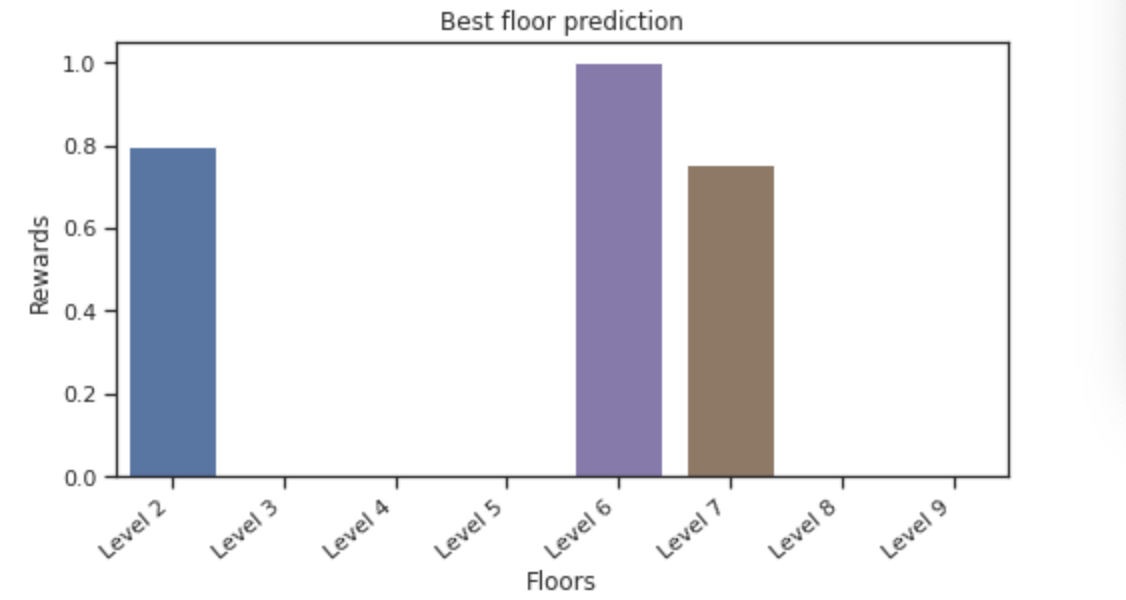
\includegraphics[width=8cm]{content/results/floors/plots/edu-floor-no-factors.png}
% \caption{Best rewarding floors from 100 Leicester St}
% \label{fig:edu-floor-no-factors}
% \end{figure}

% \item \textbf{Best nearby floors under COVID-19 Strict Lockdown:} As shown in the Appendix Table \ref{appendix:edu_mr_floor} with COVID-19 high factor, a staff member needs to walk at least \texttt{1 level} (Budget) in 100 Leicester St to get rewarding floors under  COVID-19 lockdown with the relaxing budget ($\delta$) of \texttt{5 levels} so that employee doesn't miss out a high supply providing floors. Using these constraints, we suggest \texttt{level 2} as the most rewarding floor with the cost of \texttt{1 floor} followed by \texttt{level 6} with \texttt{5 floors} and \texttt{level 7} with \texttt{6 floors} as shown in the Figure \ref{fig:edu-floor-covid}.

% \begin{figure}[H]
% \centering
%   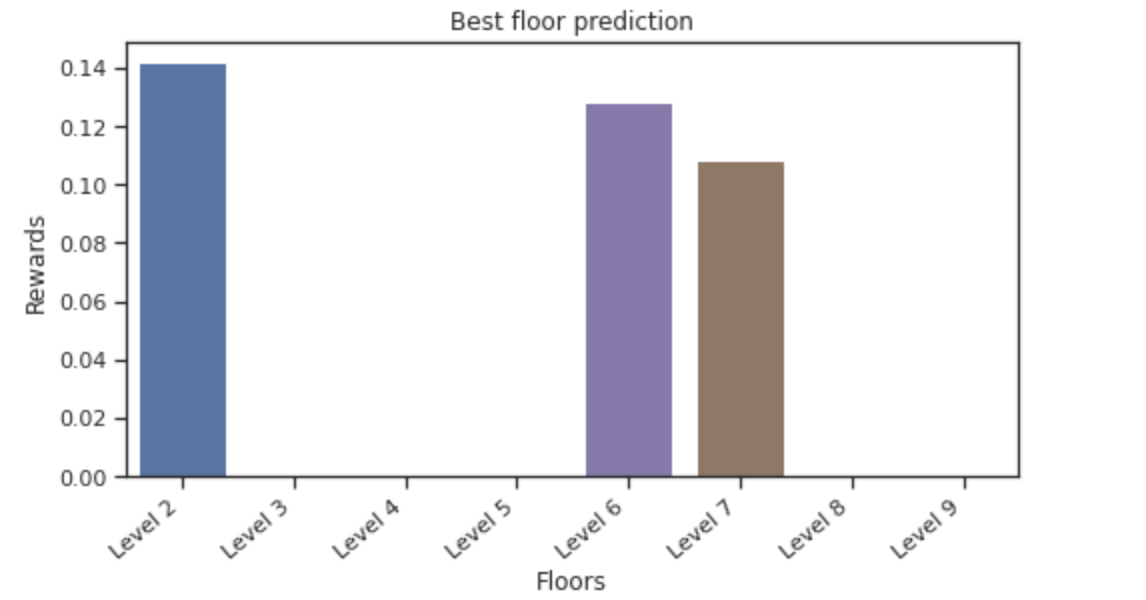
\includegraphics[width=8cm]{content/results/floors/plots/edu-floor-covid.png}
% \caption{Best rewarding floors from 100 Leicester St with COVID lockdown}
% \label{fig:edu-floor-covid}
% \end{figure}

% \item \textbf{Best nearby floors with equipment:} As shown in the Appendix Table \ref{appendix:edu_mr_floor} with equipment factor, a staff member needs to walk at least \texttt{1 level} (Budget) in 100 Leicester St to get rewarding floors to have an excellent meeting room with a relaxing budget ($\delta$) of \texttt{5 levels} so that employee doesn't miss out a high supply providing floors. Using these constraints, we suggest \texttt{level 6} as the most rewarding floor with the cost of \texttt{5 floors} followed by \texttt{level 4} with \texttt{3 floors} and \texttt{level 2} with \texttt{1 floor} as shown in the Figure \ref{fig:edu-floor-equipment}.

% \begin{figure}[H]
% \centering
%   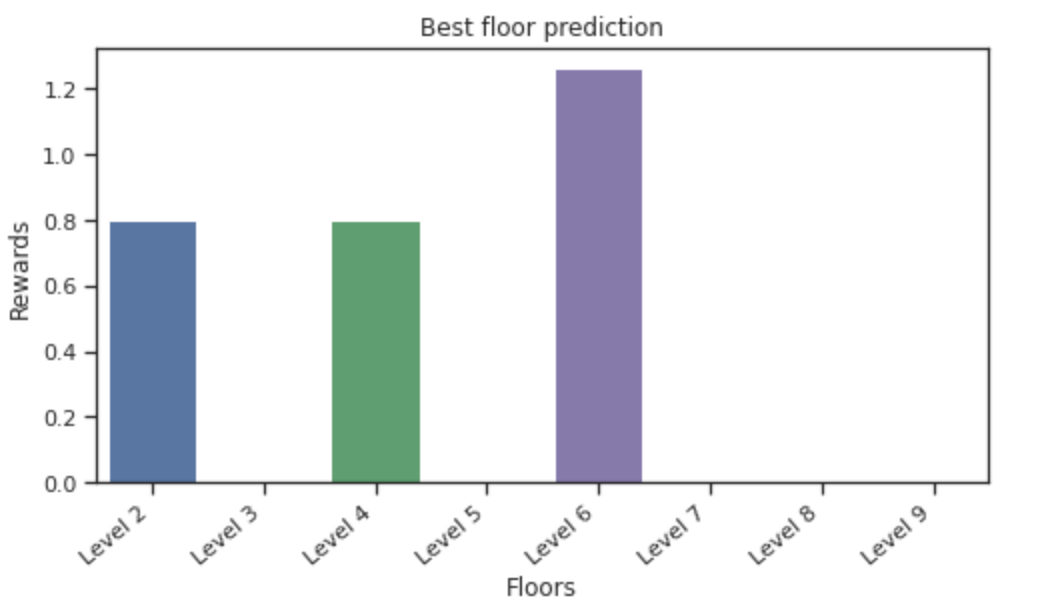
\includegraphics[width=8cm]{content/results/floors/plots/edu-floor-equipment.png}
% \caption{Best rewarding floors from 100 Leicester St with equipment}
% \label{fig:edu-floor-equipment}
% \end{figure}

% \item \textbf{Best nearby floors with other factors:} In the appendix Table \ref{appendix:edu_mr_floor}, we have also shown other factors such as finding meeting rooms with high capacity, excellent room condition, and easy availability with their budgets and relaxing budgets. Using those constraints, we suggest that \texttt{level 6} is the most rewarding floor for excellent meeting room and easy availability, \texttt{level 9} is the most rewarding floor for high capacity.

% \begin{figure}[H]
% \centering
% \begin{subfigure}[b]{0.30\textwidth}
%   \centering
%   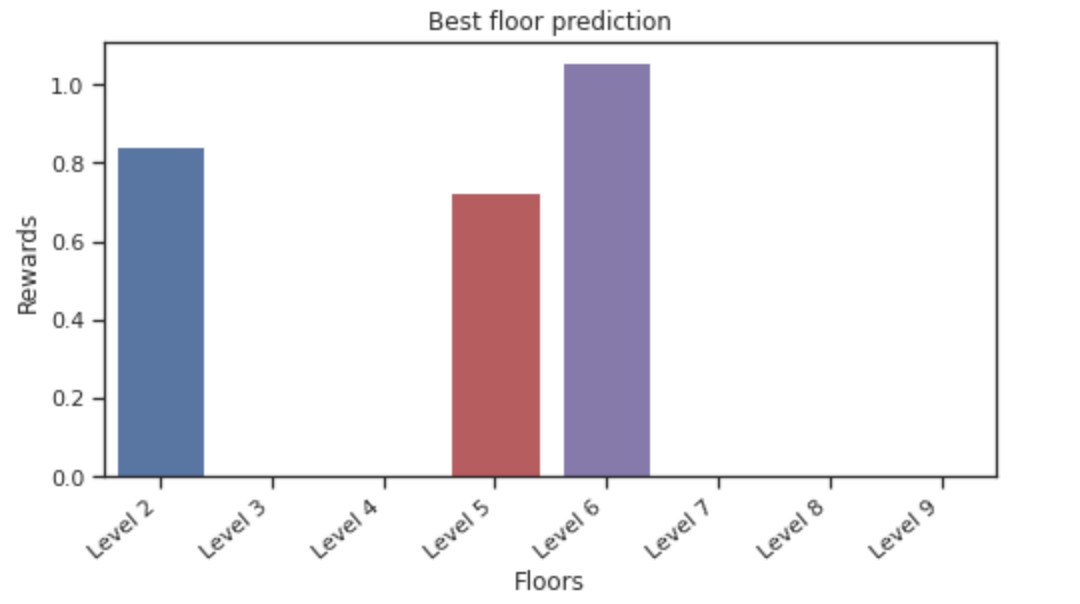
\includegraphics[width=5.5cm,keepaspectratio=true]{content/results/floors/plots/edu-floor-excellent.png}
% \end{subfigure}
% \begin{subfigure}[b]{0.30\textwidth}
%   \centering
%   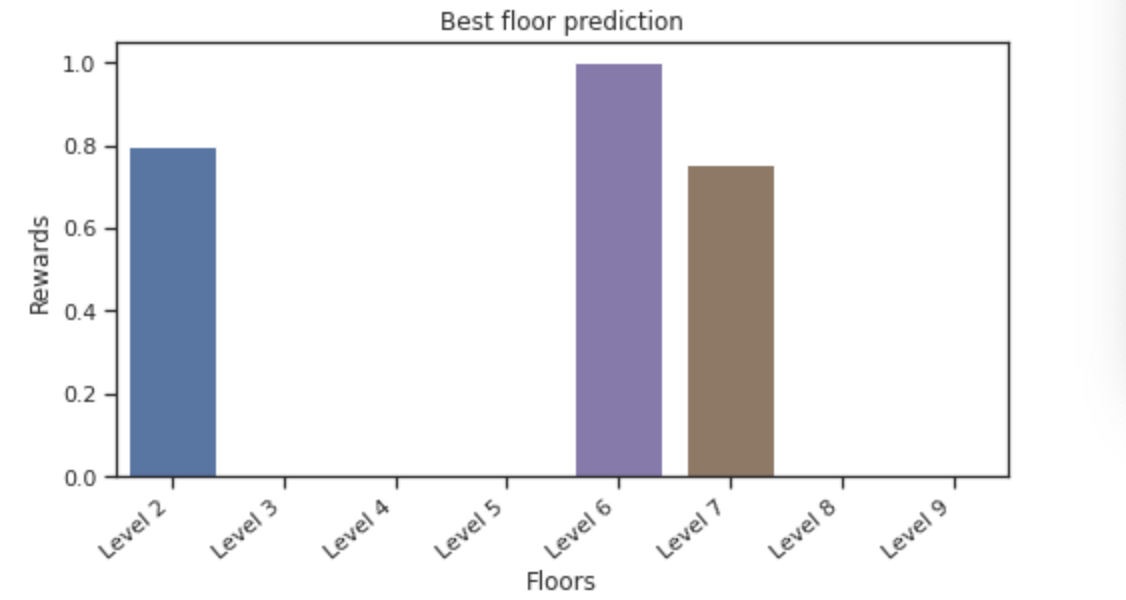
\includegraphics[width=5.5cm,keepaspectratio=true]{content/results/floors/plots/edu-floor-no-factors.png}
% \end{subfigure}
% \begin{subfigure}[b]{0.30\textwidth}
%   \centering
%   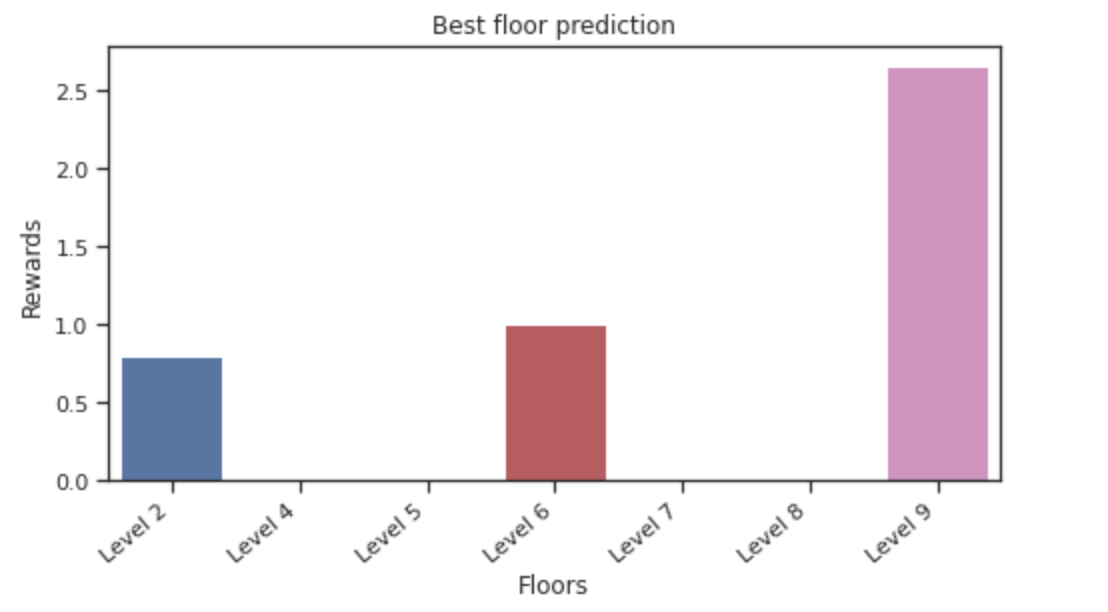
\includegraphics[width=5.5cm,keepaspectratio=true]{content/results/floors/plots/edu-floor-capacity.png}
% \end{subfigure}
% \caption{Best rewarding floors of nearby floors from 100 Leicester St based on different factors}
% \label{fig:edu-floor-other-factors}
% \end{figure}

% \end{itemize}


% \paragraph{Glyn Davis Building (Parkville Campus)}

% In this section, we will explain our findings of Glyn Davis Building from the perspective of supply and demand analysis.

% \begin{itemize}
%     \item \textbf{Best nearby floors with no preference:} As shown in the Appendix Table \ref{appendix:glyn_mr_floor}, a staff member needs to walk at least \texttt{1 level} (Budget) in the Glyn Davis Building to get rewarding floors with an adequate supply of meeting rooms. We also suggest a relaxing budget ($\delta$) of \texttt{2 levels} so that employee doesn't miss out on a high supply providing floors. Using these constraints, we suggest \texttt{level 4} as the most rewarding floor with the cost of \texttt{3 floors} followed by \texttt{level 3} with \texttt{2 floors} and \texttt{level 2} with \texttt{1 floors} as shown in the Figure \ref{fig:glyn-floor-no-factors}.
    
% \begin{figure}[H]

% \centering
%   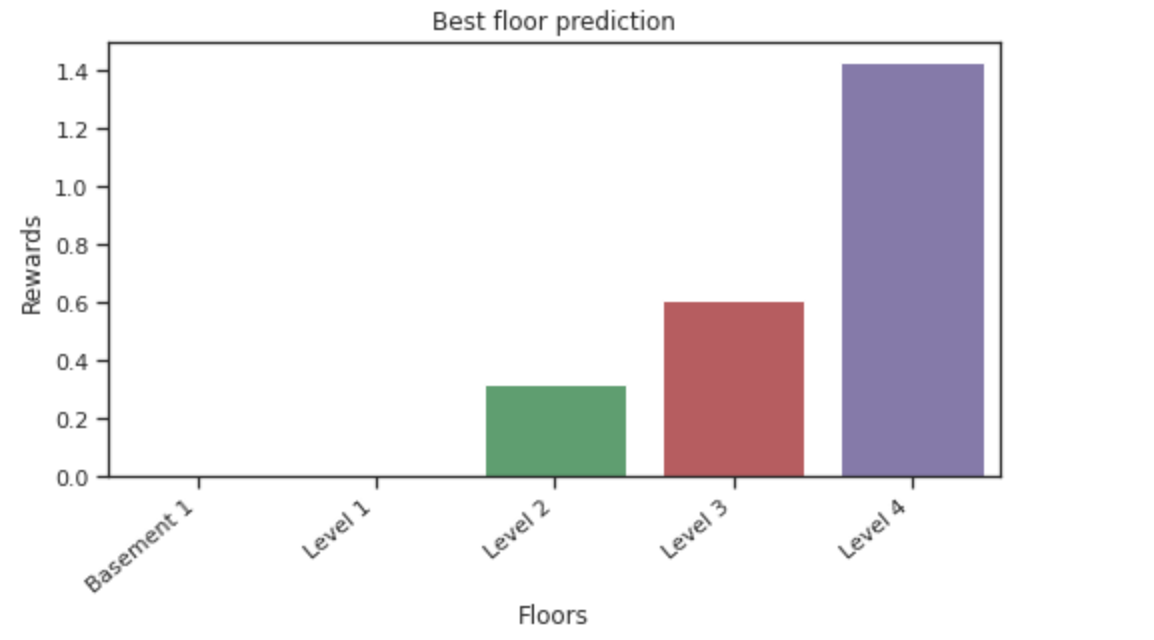
\includegraphics[width=8cm]{content/results/floors/plots/glyn-floor-no-factors.png}
  
% \caption{Best rewarding floors from Glyn Davis}
% \label{fig:glyn-floor-no-factors}
% \end{figure}

% \item \textbf{Best nearby floors under COVID-19 Strict Lockdown:} As shown in the Appendix Table \ref{appendix:glyn_mr_floor} with COVID-19 high factor, a staff member should be willing to walk at least \texttt{1 level} (Budget) in Glyn Davis Building to get very high rewarding floors under COVID-19 lockdown with the relaxing budget($\delta$) of at least \texttt{2 levels}. Using these constraints, we suggest \texttt{level 4} as the most rewarding floor with the cost of \texttt{3 floors} followed by \texttt{level 3} with \texttt{2 floors} and \texttt{Basement 1} with \texttt{0.9 floor} as shown in the Figure \ref{fig:glyn-floor-covid}.

% \begin{figure}[H]
% \centering
%   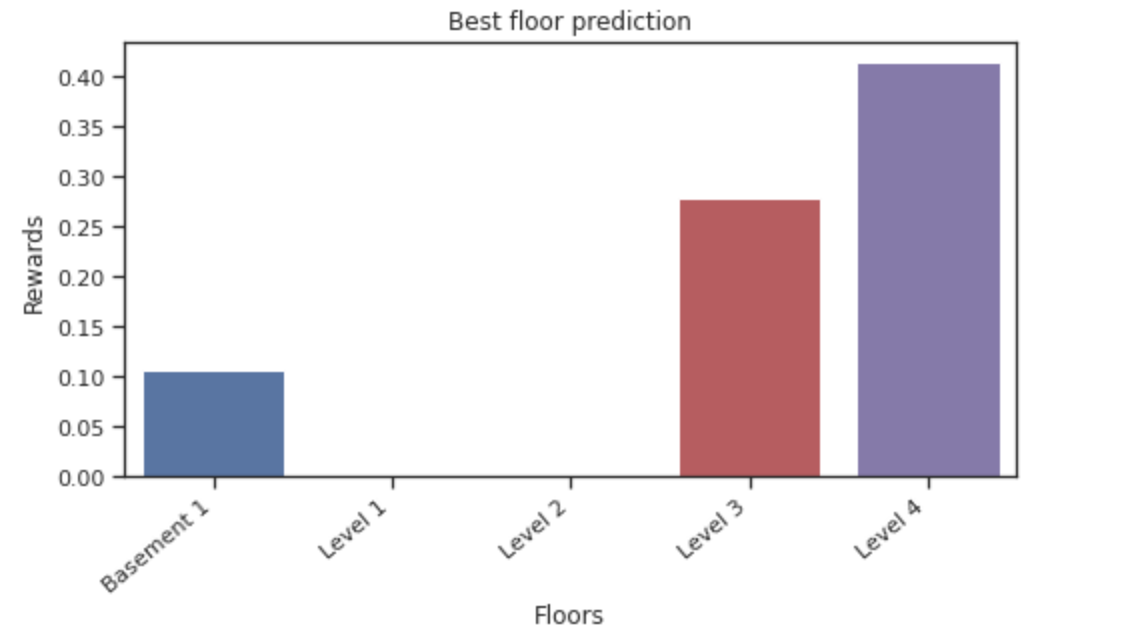
\includegraphics[width=8cm]{content/results/floors/plots/glyn-floor-covid.png}
  
% \caption{Best rewarding floors from Glyn Davis with COVID lockdown}
% \label{fig:glyn-floor-covid}
% \end{figure}

% \item \textbf{Best nearby floors with High Capacity:} As shown in the Appendix Table \ref{appendix:glyn_mr_floor} with high capacity factor, a staff member can easily find high supply of meeting rooms providing floors in Glyn Davis building within the budget of \texttt{1 level} and relaxing budget($\delta$) of at least \texttt{2 levels}. Using these constraints, we again suggest \texttt{level 4} as the most rewarding floor with the cost of \texttt{3 floors} followed by \texttt{level 3} with \texttt{2 floors} and \texttt{Basement 1} with \texttt{0.9 floor} as shown in the Figure \ref{fig:glyn-floor-capacity}.

% \begin{figure}[H]
% \centering
%   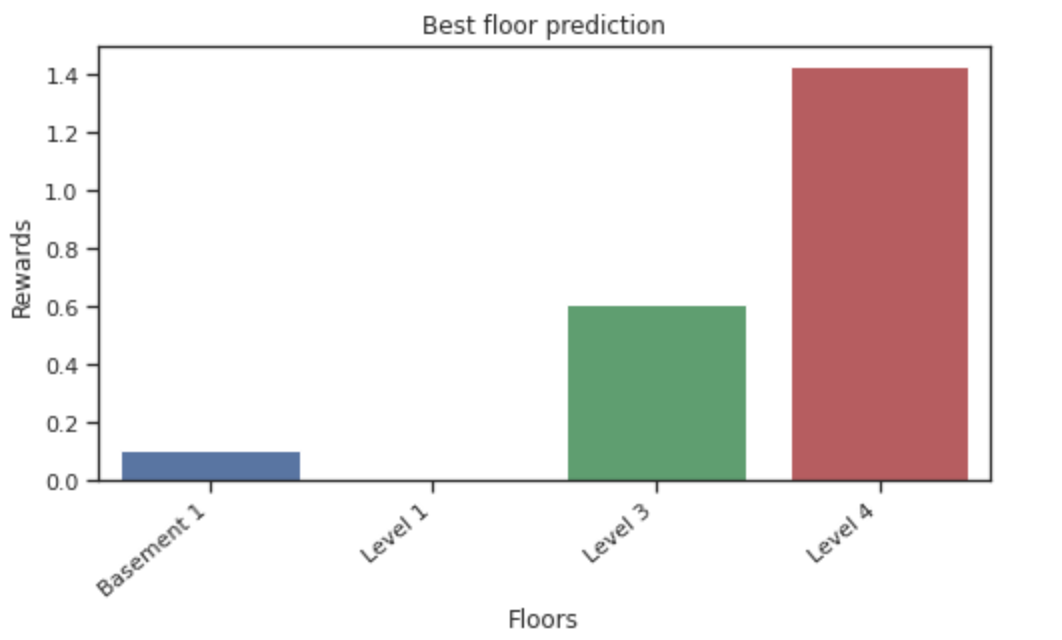
\includegraphics[width=8cm]{content/results/floors/plots/glyn-floor-capacity.png}
% \caption{Best rewarding floors from Glyn Davis with high capacity}
% \label{fig:glyn-floor-capacity}
% \end{figure}

% \item \textbf{Best nearby floors with other factors:} In the appendix Table \ref{appendix:glyn_mr_floor}, we have also shown other factors such as finding meeting rooms with equipment, excellent conditions, and easy availability with their budgets and relaxing budgets. Using those constraints, we suggest that \texttt{level 4} is the most rewarding floor for meeting rooms for those factors.

% \begin{figure}[H]
% \centering
%   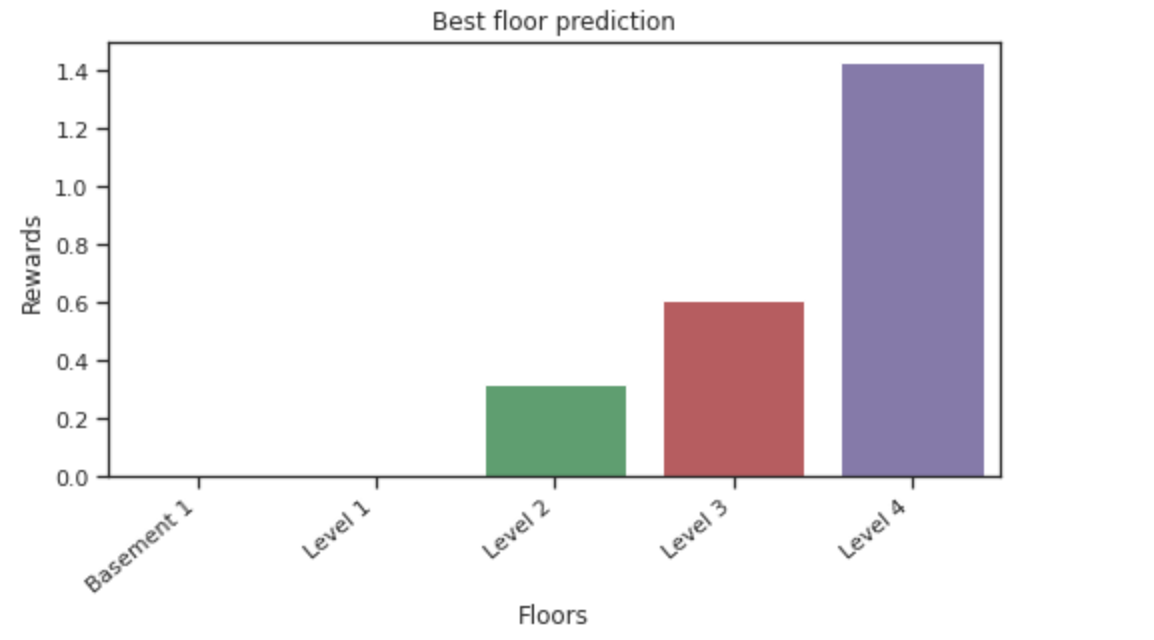
\includegraphics[width=8cm]{content/results/floors/plots/glyn-floor-no-factors.png}
% \caption{Best rewarding floors from Glyn Davis with other factors}
% \label{fig:glyn-floor-other-factors}
% \end{figure}

% \end{itemize}



\paragraph{Elisabeth Murdoch Building (Southbank Campus)}
In this section, we will explain our findings of Elisabeth Murdoch Building from the perspective of supply and demand analysis.

\begin{itemize}
    \item \textbf{Best nearby floors with no preference:} As shown in the Appendix Table \ref{appendix:eliz_mr_floor}, a staff member needs to walk at least \texttt{1 level} (Budget) in Elisabeth Murdoch Building to get rewarding floors with an adequate supply of meeting rooms. We also suggest a relaxing budget ($\delta$) of \texttt{1 level} so that employee doesn't miss out a high supply providing floors. Using these constraints, we suggest \texttt{level 3} as the most rewarding floor with the cost of \texttt{2 floors} followed by \texttt{level 2} with \texttt{1 floor} as shown in the Figure \ref{fig:eliz-floor-no-factors}.

\begin{figure}[H]
\centering
  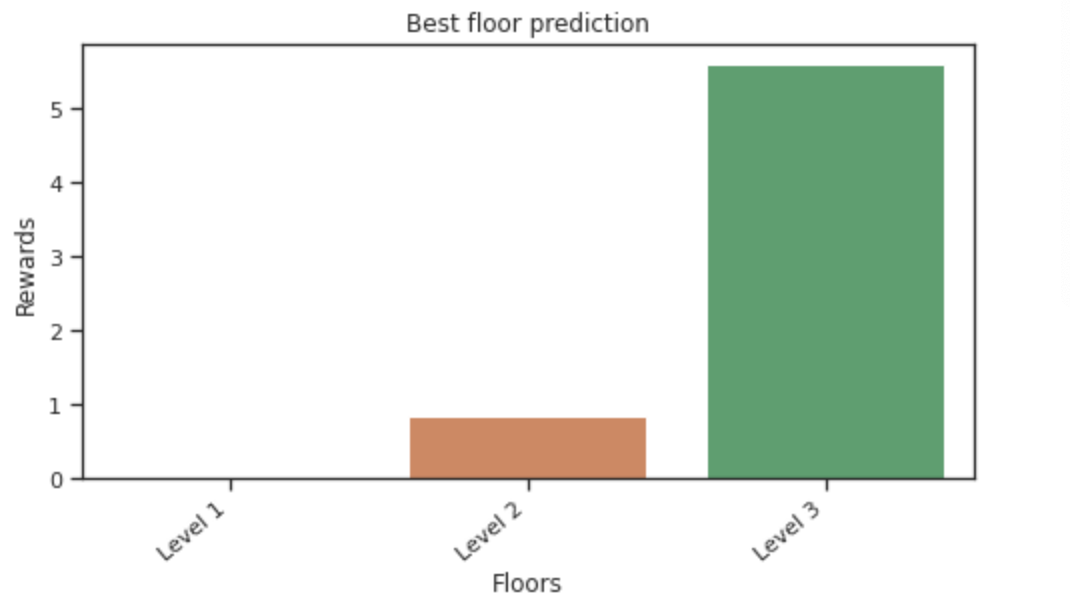
\includegraphics[width=8cm]{content/results/floors/plots/eliz-floor-no-factors.png}
\caption{Best rewarding floors from Elisabeth Murdoch Building}
\label{fig:eliz-floor-no-factors}
\end{figure}

%\item \textbf{Best nearby floors under COVID-19 Strict Lockdown:} As shown in the Appendix Table \ref{appendix:eliz_mr_floor} with COVID-19 high factor, a staff member needs to walk at least \texttt{1 level} (Budget) in Elisabeth Murdoch Building to get rewarding floors under  COVID-19 lockdown with the relaxing budget ($\delta$) of \texttt{1 level} so that employee doesn't miss out a high supply providing floors. Using these constraints, we suggest \texttt{level 3} as the most rewarding floor with the cost of \texttt{2 floors} followed by \texttt{level 2} with \texttt{1 floor} as shown in the Figure \ref{fig:eliz-floor-covid}.

%\begin{figure}[H]
%\centering
%  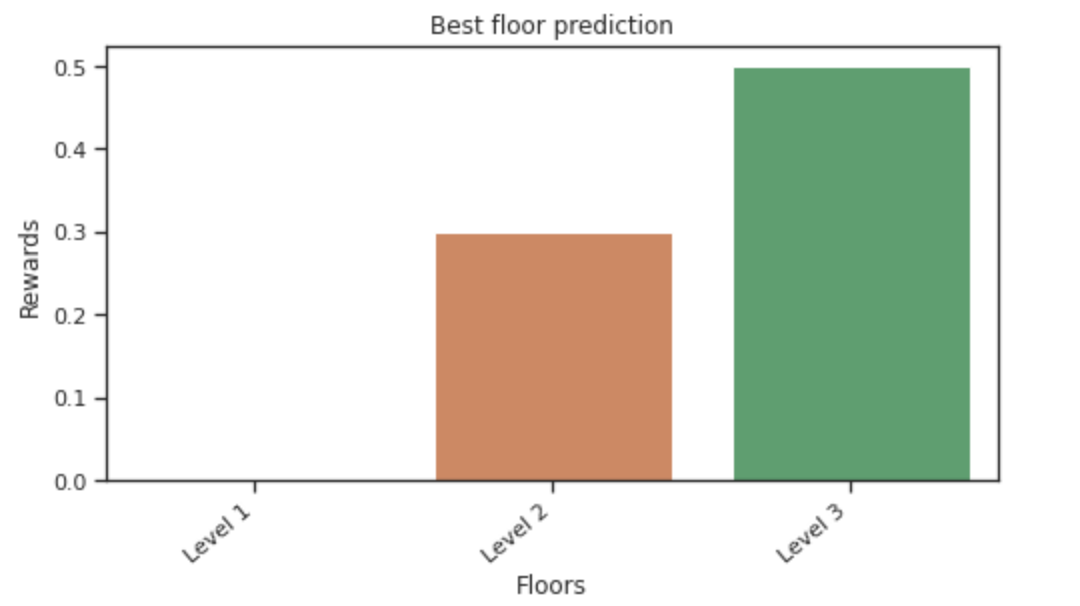
\includegraphics[width=8cm]{content/results/floors/plots/eliz-floor-covid.png}
%\caption{Best rewarding floors from Elisabeth Murdoch Building with COVID lockdown}
%\label{fig:eliz-floor-covid}
%\end{figure}

\item \textbf{Best nearby floors with equipment:} As shown in the Appendix Table \ref{appendix:eliz_mr_floor} with equipment factor, a staff member needs to walk at least \texttt{1 level} (Budget) in Elisabeth Murdoch Building to get rewarding floors to have an excellent meeting room with the relaxing budget ($\delta$) of \texttt{1 level} so that employee doesn't miss out a high supply providing floors. Using these constraints, we suggest \texttt{level 2} as the most rewarding floor with the cost of \texttt{1 floor} followed by \texttt{level 3} with \texttt{2 floors} as shown in the Figure \ref{fig:eliz-floor-equipment}.

\begin{figure}[H]
\centering
  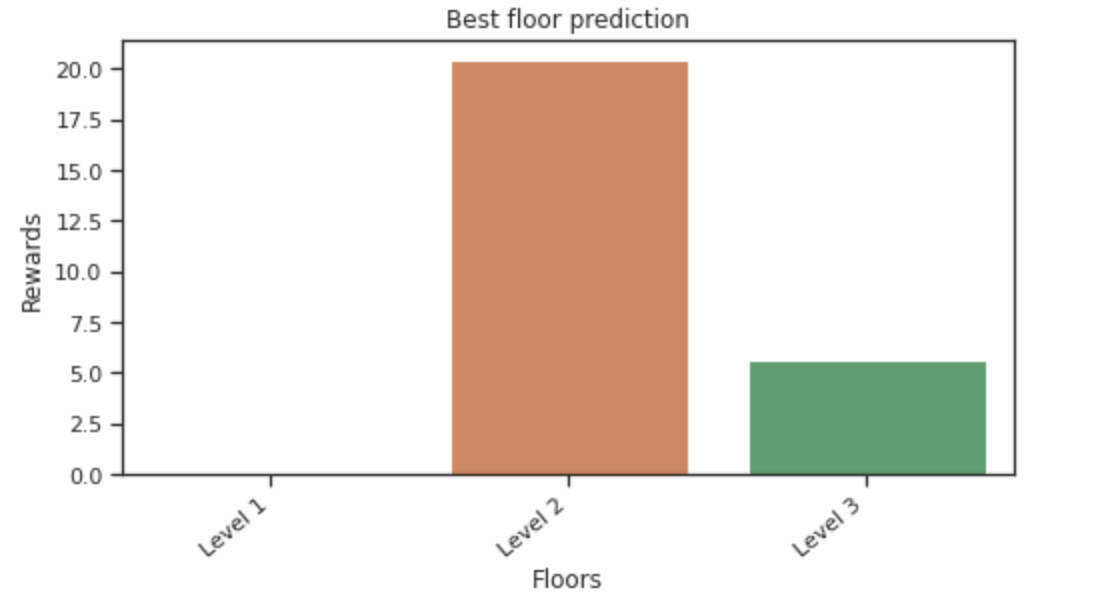
\includegraphics[width=8cm]{content/results/floors/plots/eliz-floor-equipment.png}
\caption{Best rewarding floors from Elisabeth Murdoch Building with equipment}
\label{fig:eliz-floor-equipment}
\end{figure}

\item \textbf{Best nearby floors with other factors:} In the appendix Table \ref{appendix:eliz_mr_floor}, we have also shown other factors such as finding meeting rooms with high capacity, excellent room condition, and easy availability with their budgets and relaxing budgets. Using those constraints, we suggest that \texttt{level 3} is the most rewarding floor for all factors.

\begin{figure}[H]
\centering
  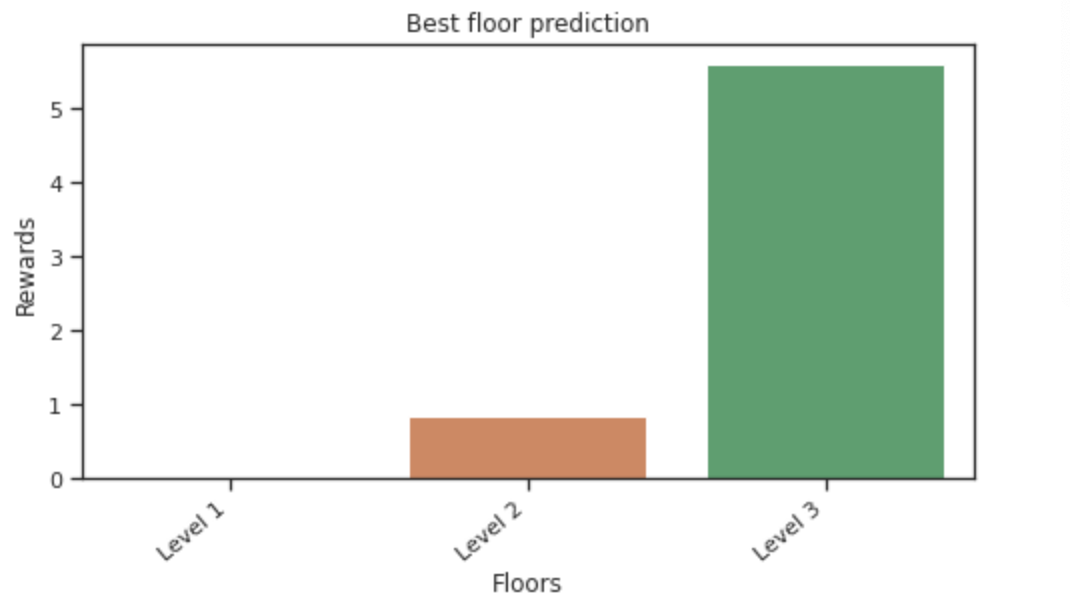
\includegraphics[width=8cm]{content/results/floors/plots/eliz-floor-no-factors.png}
\caption{Best rewarding floors from Elisabeth Murdoch Building with other factors}
\label{fig:eliz-floor-other-factors}
\end{figure}
\end{itemize}


% 
%\paragraph{Werribee Veterinary Hospital (Werribee Campus)}
% In this section, we will explain our findings of Werribee Veterinary Hospital from the perspective of supply and demand analysis. 
% \newline

% \noindent
% As shown in the Appendix Table \ref{appendix:werribee_mr_floor}, a staff member needs to walk at least \texttt{1 level} (Budget) in Werribee Veterinary Hospital to get rewarding floors with an adequate supply of meeting rooms. As there is only one floor that has a meeting room, all factors will not change our prediction to find the best floor. The Ground floor is the only solution for this building as shown in the Figure \ref{fig:werribee-floor-no-factors}.

% \begin{figure}[H]
% \centering
%   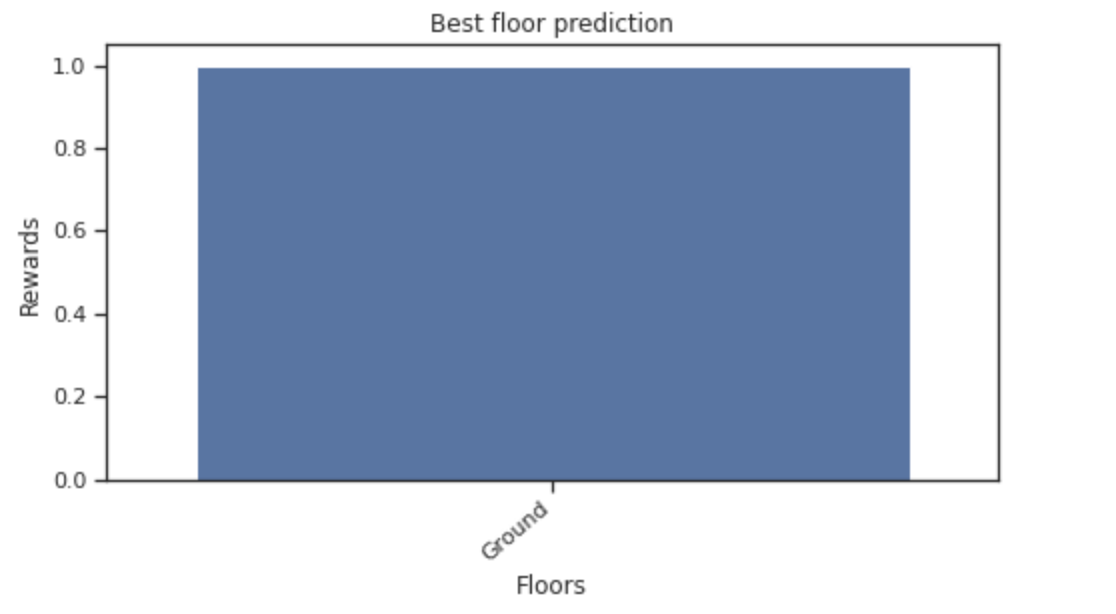
\includegraphics[width=8cm]{content/results/floors/plots/werribee-floor-no-factors.png}
% \caption{Best rewarding floors from Werribee Veterinary Hospital}
% \label{fig:werribee-floor-no-factors}
% \end{figure}